\Chapter{Experimental Set Up}

\Section{Introduction}

Before final experimental measurements can be done, 
a fair amount of set up and preliminary measurements must be made and understood. 
In this chapter, a some background information on the facility will be presented, 
including the changes required  to achieve fully independent staging.
The laser pulse train generated at the facility was measured and improved 
through the characteristics of the ultraviolet optics being used. 
RF measurements were done to understand the power distribution in the gun and linac.
Several beam diagnostics are introduced, such as beam size measurements using 
florescent screens, bunch length measurements using coherent transition radiation, 
and energy measurements using a dipole spectrometer. 
Finally a review of the design requirements for fully staged TBA is discussed.

%%%%%%%%%%%%%%%%%%%%%%%%%%%%%%%%%%%%%%%%%%%%%%%%%%%%%%%%%%%%%%%%%%%%%%%%%%%%%%%%
%%%%%%%%%%%%%%%%%%%%%%%%%%%%%%%%%%%%%%%%%%%%%%%%%%%%%%%%%%%%%%%%%%%%%%%%%%%%%%%%
\Section{Argonne Wakefield Accelerator Facility} \label{sec:facility}
%%%%%%%%%%%%%%%%%%%%%%%%%%%%%%%%%%%%%%%%%%%%%%%%%%%%%%%%%%%%%%%%%%%%%%%%%%%%%%%%
%%%%%%%%%%%%%%%%%%%%%%%%%%%%%%%%%%%%%%%%%%%%%%%%%%%%%%%%%%%%%%%%%%%%%%%%%%%%%%%%

The AWA facility houses two rf photoinjector electron guns operating
at \SI{1.3}{GHz}, and three subsequent beam lines. 
Two of the beam lines are currently used for staged TBA, and the
third is used for Emittance Exchange experiments (EEX). A layout of
the facility is shown in Figure~\ref{fig:bunker}.  
The beam to be accelerated starts at the witness gun (bottom left in Figure~\ref{fig:bunker}) 
and traverses through two accelerating structures powered by beams counter-propagating through 
an independent accelerator. The drive beam from which the energy is extracted starts at the drive gun (far right in Figure~\ref{fig:bunker}).
The layout of the drive accelerator must be changed from the current layout shown in the figure to achieve independent staging.  
It can be seen that the same drive beam bunch train passes through both decelerators, 
whereas for independent staging the decelerating structures would be powered by separate bunch trains
that are separated into independent beam lines by a fast rise time kicker and septum, see Figure~\ref{fig:singlestage}. 
\begin{figure}
	\begin{center}
		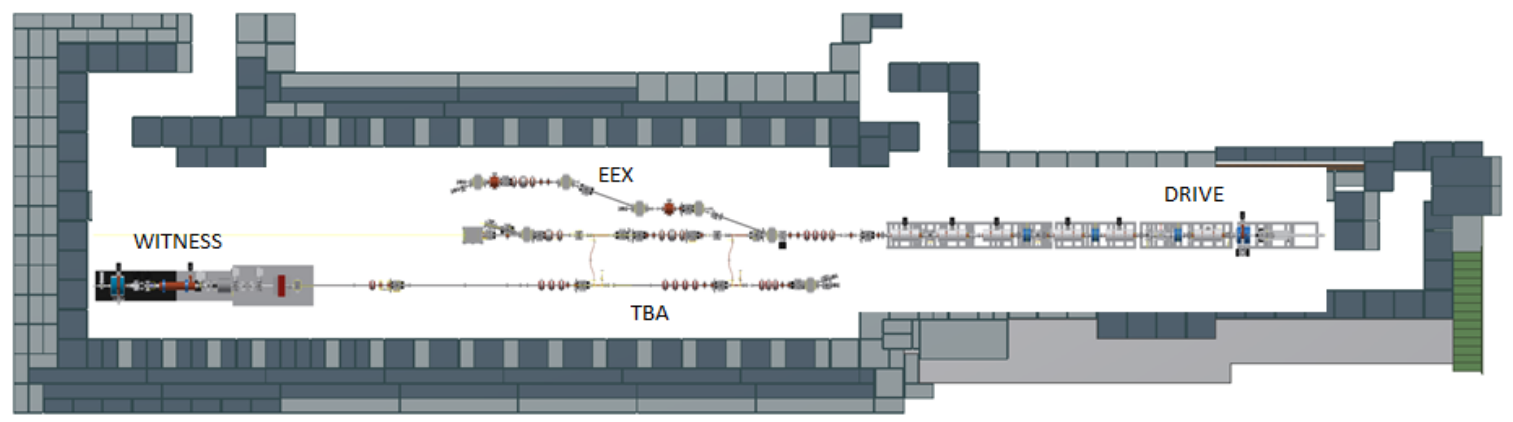
\includegraphics[width=\linewidth]{./images/bunker}
	\end{center}
	\caption{AWA Facility bunker and simplified TBA staging layout. 
		The drive beam line (right) supplies high charge bunch trains at \SI{70}{MeV}.
		The witness beam line (left) supplies low charge one bunch at \SI{15}{MeV}. 
		CAD drawing of bunker courtesy of Scott Doran at AWA.}
	\label{fig:bunker}
\end{figure}
\begin{figure}
	\begin{center}
		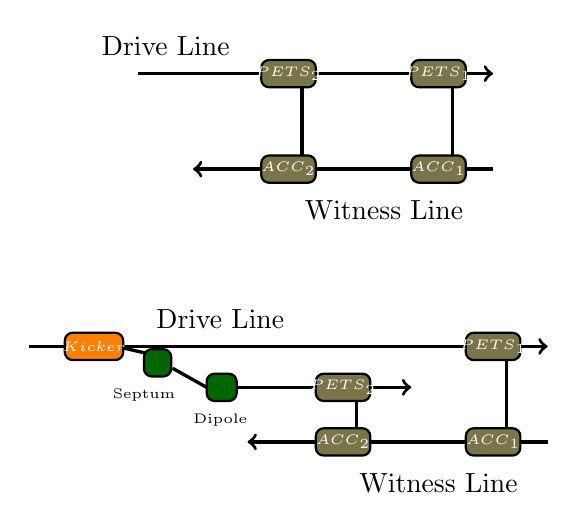
\begin{tikzpicture}[scale=\textwidth/35cm, text=black]
		\def \gunleft {-1.0}
\def \gunright {0.3}
\def \loneright {1.0}
\def \ltworight {2.0}
\def \lthreeright {3.0}
\def \lfourright {4.0}
\def \lfiveright {5.0}
\def \lsixright {6.0}
\def \quadone {7.3}
\def \quadfour{16}

%Full Staging
\draw[very thick, ->] (8,1) -- (27,1);

%Line between kicker and septum
\node[] at (15,2) {Drive Line};
\node[] at (23,-4) {Witness Line};
\draw[very thick] (\lsixright+5.2,1.0) -- (12.5,0.7);

%Kicker 
\draw[fill=orange,  thick, rounded corners =0.1cm] (\lsixright+3.3,0.5)rectangle ({\lsixright+0.84+4.6},1.5) node[pos=.5, white] {\tiny $Kicker$};
%Septum
\node[] at (12.2,-0.8) {\tiny Septum};
\draw[fill=black!60!green,  thick, rounded corners =0.1cm] (12.2,0.9)rectangle ({13.2},-0.1) node[pos=.5, white] {};
%Line between kicker and septum
\draw[very thick] (13.25,0.2) -- (14.5,-0.5);
%Dipole
\node[] at (15,-1.7) {\tiny Dipole};
\draw[fill=black!60!green, thick, rounded corners =0.1cm] (14.5,0.0)rectangle ({15.6},-1.0) node[pos=.5, white] {};
%Line between dipole and quads
\draw[very thick, ->] (15.6,-0.5) -- (22,-0.5);
%Witness
\draw[very thick, <-] (16,-2.5) -- (27,-2.5);
%Waveguide
\draw[very thick] (20,-0.5) -- (20,-3);
%Waveguide
\draw[very thick] (25.5,1.5) -- (25.5,-3);
%PETS2
\draw[fill=black!60!yellow,  thick, rounded corners =0.1cm] (18.5,0.0)rectangle (20.5,-1) node[pos=.5, white] {\tiny$\text{PETS}_2$};
%PETS1
\draw[fill=black!60!yellow,  thick, rounded corners =0.1cm] (24,1.5)rectangle (26,0.5) node[pos=.5, white] {\tiny$\text{PETS}_1$};
%ACC2
\draw[fill=black!60!yellow,  thick, rounded corners =0.1cm] (18.5,-2)rectangle (20.5,-3) node[pos=.5, white] {\tiny$\text{ACC}_2$};
%ACC1
\draw[fill=black!60!yellow,  thick, rounded corners =0.1cm] (24,-2)rectangle (26,-3) node[pos=.5, white] {\tiny$\text{ACC}_1$};



%Simplified Staging



\draw[very thick, ->] (12,11) -- (25,11);

%Line between kicker and septum
\node[] at (13,12) {Drive Line};
\node[] at (21,6) {Witness Line};

%Witness
\draw[very thick, <-] (14,10-2.5) -- (25,10-2.5);
%Waveguide
\draw[very thick] (18,11.5) -- (18,7);
%Waveguide
\draw[very thick] (23.5,11.5) -- (23.5,10-3);
%PETS2
\draw[fill=black!60!yellow,  thick, rounded corners =0.1cm] (16.5,11.5)rectangle (18.5,10.5) node[pos=.5, white] {\tiny$\text{PETS}_2$};
%PETS1
\draw[fill=black!60!yellow,  thick, rounded corners =0.1cm] (22,11.5)rectangle (24,10.5) node[pos=.5, white] {\tiny$\text{PETS}_1$};
%ACC2
\draw[fill=black!60!yellow,  thick, rounded corners =0.1cm] (16.5,8)rectangle (18.5,7) node[pos=.5, white] {\tiny$\text{ACC}_2$};
%ACC1
\draw[fill=black!60!yellow,  thick, rounded corners =0.1cm] (22,8)rectangle (24,7) node[pos=.5, white] {\tiny$\text{ACC}_1$};








		\end{tikzpicture}
	\end{center}
	\caption{Simplified drawing of the two staging schemes.
		No quadrupole elements are included, and the arrows indicate what direction the beams travels.
		PETS stands for Power Extraction and Transfer Structure, and ACC stands for Accelerating structure. 
		The subscript on each structure refers to which stage the structures belong to (first or second). 
		In the simplified staging scheme the stages are not separated, meaning bunch train two travels
		through and loses energy in the first stage before reaching the second stage.
		This is prevented by separate beam lines in the full staging layout. }
	\label{fig:singlestage}
\end{figure}

Electron bunches in a photoinjector are created through the photoelectric effect. 
At the AWA, a pulsed UV laser is propagated through two relay lines of UV optics to either
the drive or witness gun. An in-vacuum mirror then directs the pulse to the photocathode.
Both beam lines must be operated simultaneously when the TBA experiments are run. This is accomplished by
splitting the original laser pulse into two pulses using a UV splitter on the 
ceiling of the bunker. One of the split pulses is sent (as is) to the witness beam line for one
bunch operation. The second pulse is sent to a UV multispitter table, shown in 
Figure~\ref{fig:optics} where it is split into trains of various lengths. Eight pulses are 
used for TBA drive trains,

The rf photoinjector on the drive line uses a semiconducting
cesium telluride (CsTe) cathode, and is followed by a linear accelerator (linac). The
drive linac uses six copper cavities and four klystrons to accelerate the drive beam
to energies of 50-\SI{70}{MeV}. The number of bunches generated from each 
laser pulse can vary from 1, 2, 4, 6, and 8 bunches. When multiple bunches
are generated, the grouping is called a bunch train. Generation of
these variable bunch trains is accomplished by splitting the pulsed
UV laser beam before it enters the gun and hits the cathode. The splitting
takes place in a complex network of UV optics located near the drive
gun. The optics set up is called a beam splitter, or mulitsplitter,
and trains are created at a rate of 0.5, 1, or \SI{2}{Hz}. 
This timing is the repetition rate of the machine. 
A simplified diagram of this is timing is shown in Figure~\ref{fig:lasertiming}, 
and a picture of the AWA multisplitter table is shown in Figure~\ref{fig:optics}. 
Optimization of the UV optics was performed and is detailed in Section \ref{sec:uvoptics}.  
\begin{figure}
	\centering
	\begin{tikzpicture}[every node/.style={anchor=south west,inner sep=0pt},x=1mm, y=1mm,]   
	\node (fig1) at (0,0)
	{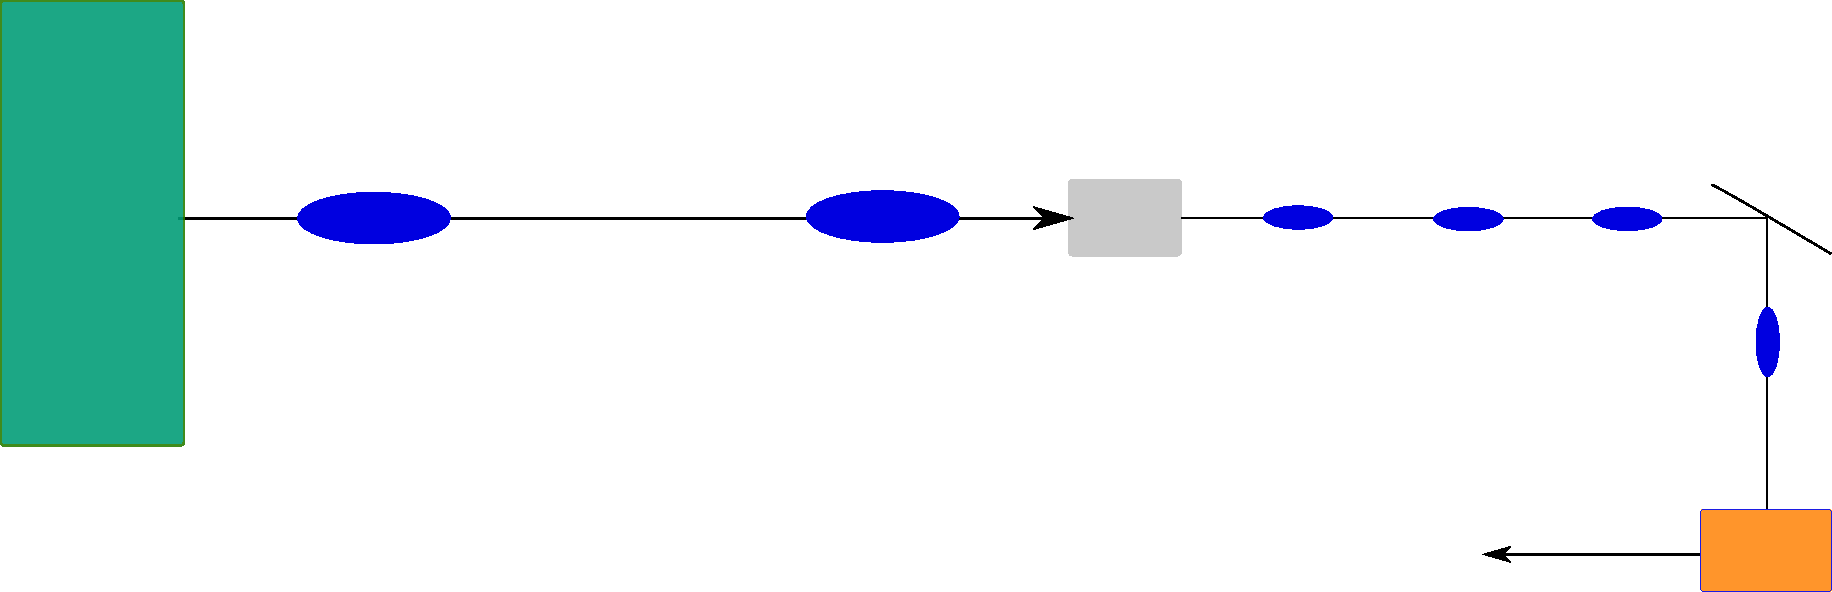
\includegraphics[width=\textwidth]{images/laserpulsetrain}};
	\node[fill=white, inner sep=2pt] (txt2) at (-2,53) {Laser room};
	\node[fill=white, inner sep=2pt] (txt2) at (20,20) {Laser pulse};	
	\node[fill=white, inner sep=2pt] (txt2) at (110,20) {Laser pulse train};
	\node[fill=white, inner sep=2pt] (txt2) at (82,35) {Multisplitter};	
	\node[fill=white, inner sep=2pt] (txt2) at (143,35) {Mirror};	
	\node[fill=white, inner sep=2pt] (txt2) at (143,-5) {Gun};
	\end{tikzpicture}
	\caption{Simplified drawing of the laser pulse as it travels to the gun.
	The spacing of the laser pulses exiting the laser room is equal to the 
	repetition rate of the machine (0.5, 1, or \SI{2}{Hz}).
	When in the multisplitter, the original laser pulse is split into a pulse train of
	2, 4, 8, or 16 pulses. 
	The intensity of original laser pluse is equal to the sum of all members in the pulse train.
	The spacing in the plus train is one period of the RF supplied to the cavities, w
	which is \SI{1.3}{GHz} or \SI{769}{ps}. }
	%\label{inter}
	%\caption{Bolometer. }
	\label{fig:lasertiming}
\end{figure}
\begin{figure}%[h]
	\begin{center}
		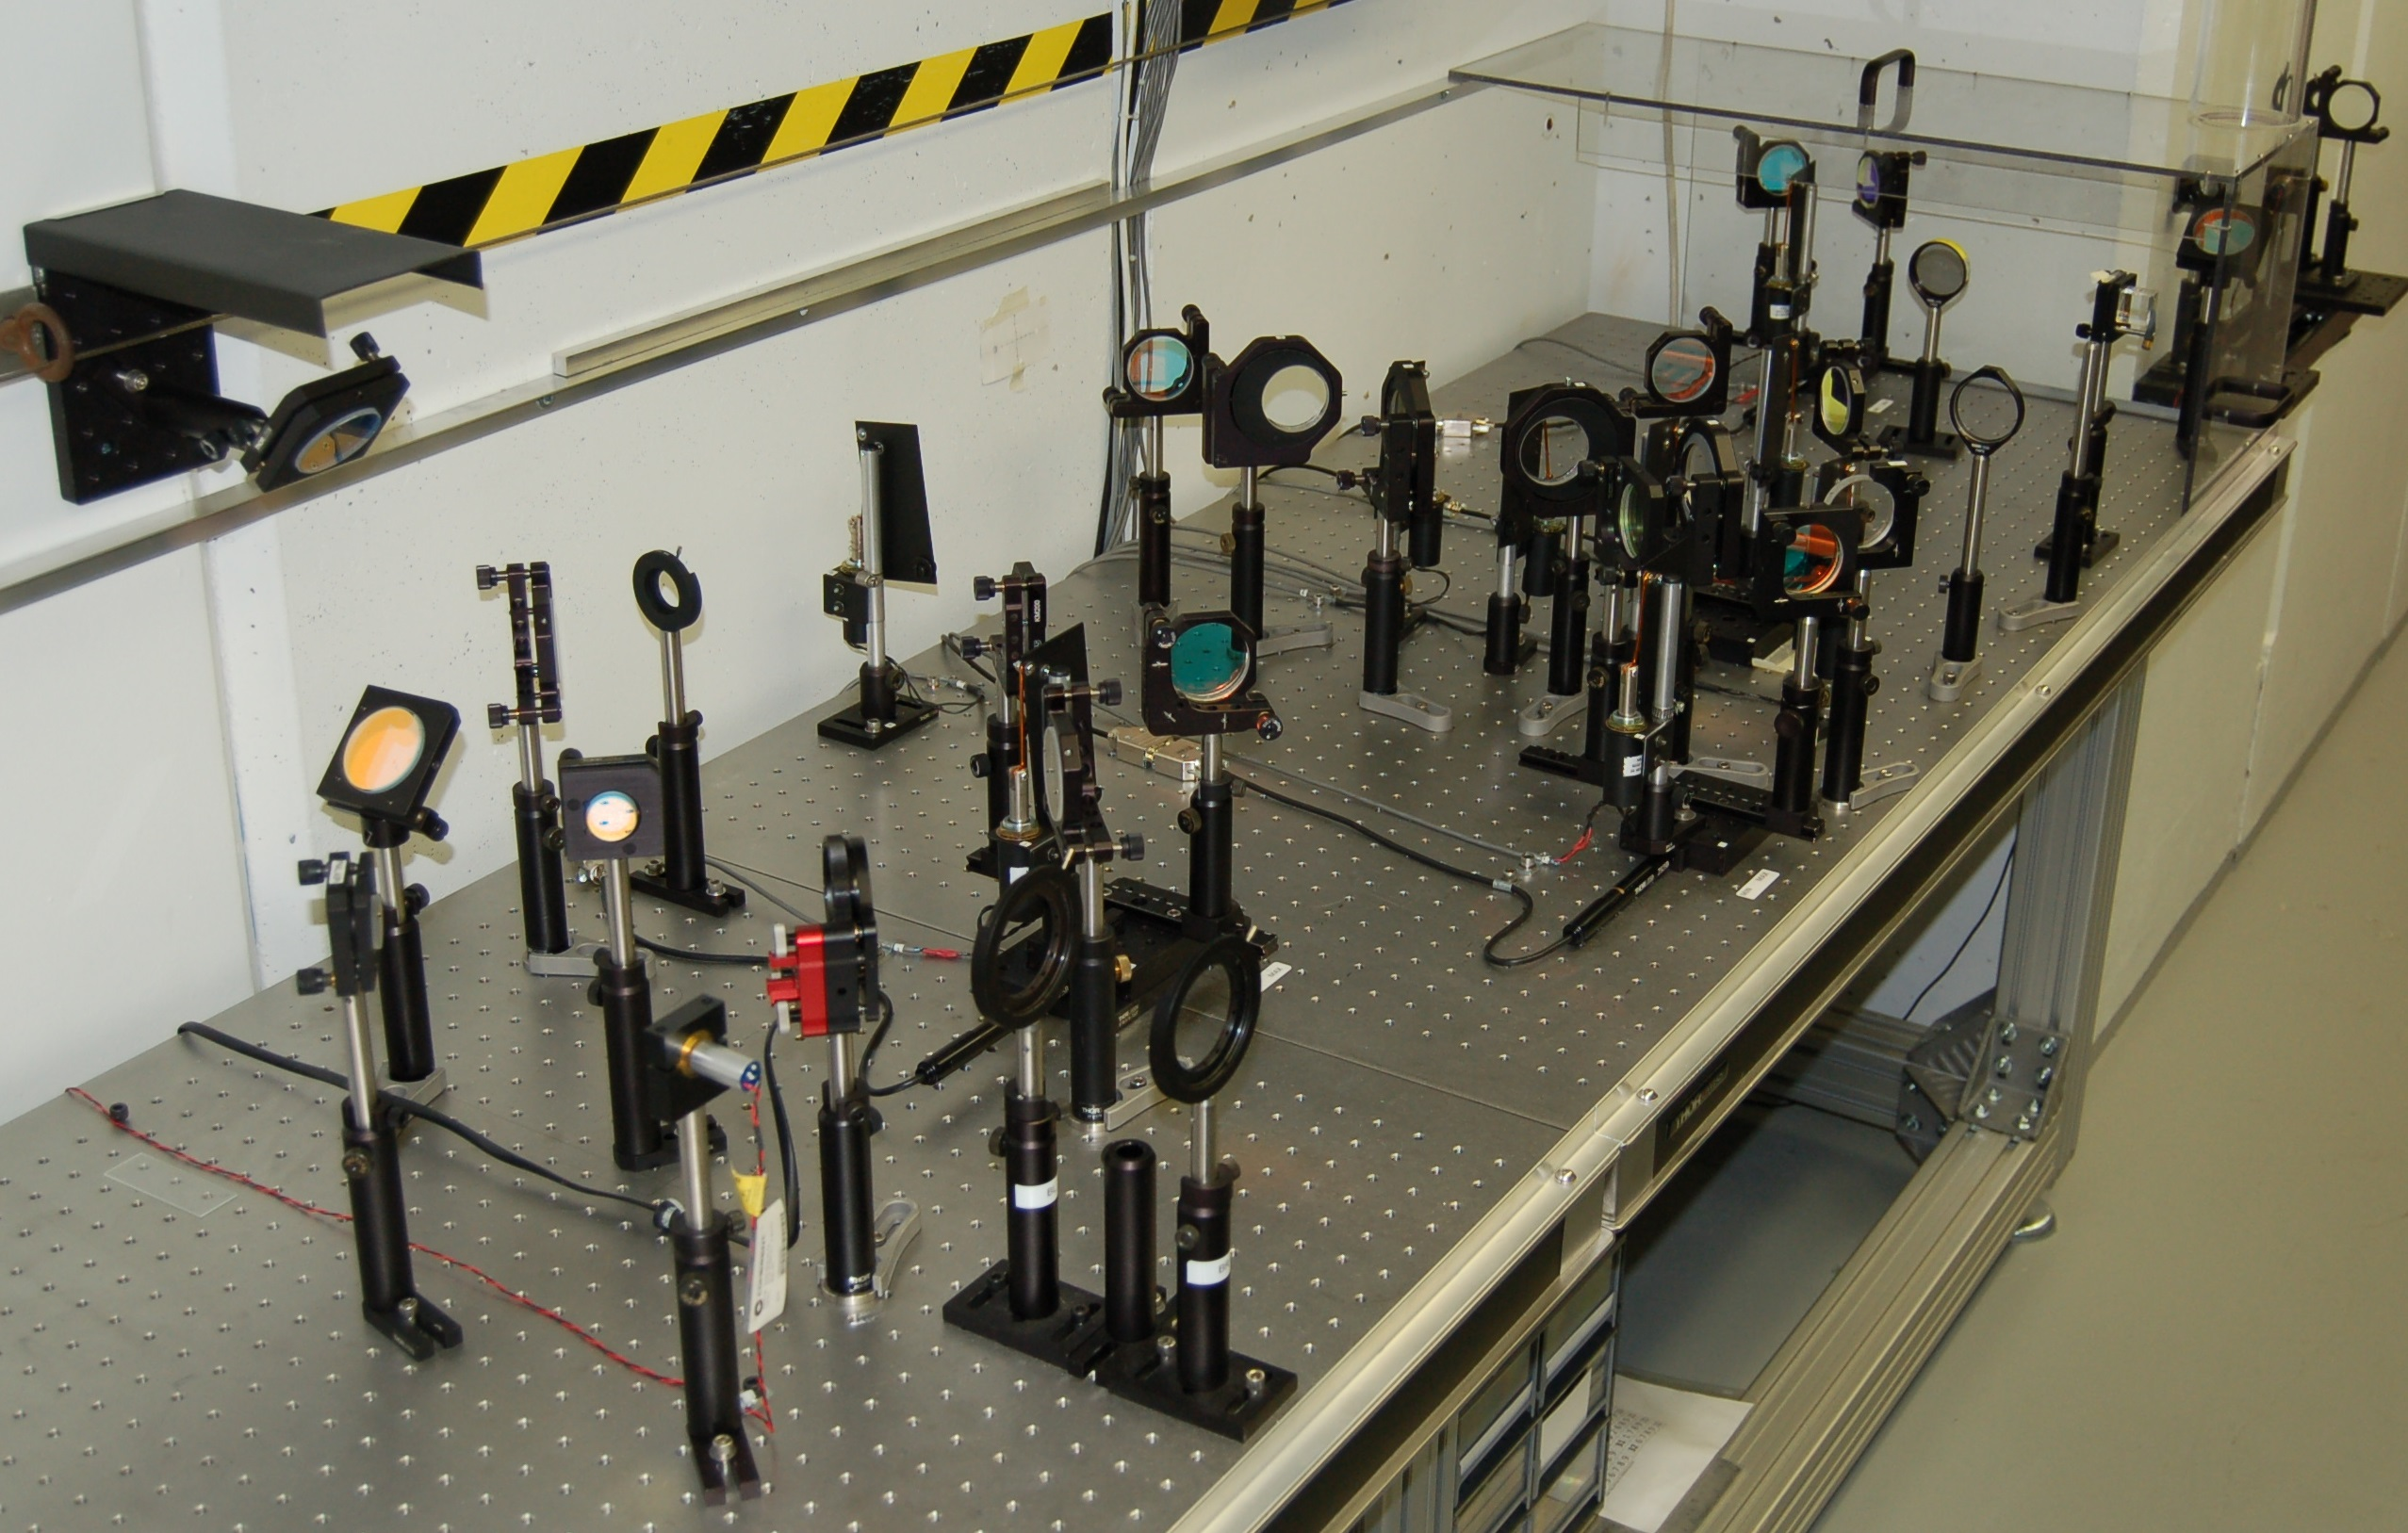
\includegraphics[width=0.5\textwidth]{images/multisplitter}
		\caption{UV multisplitter optics table.}\label{fig:optics}
	\end{center}
\end{figure}

The witness line rf photoinjector, located on the left side of Figure~\ref{fig:bunker}, 
uses a magnesium cathode and the following linac consists of one copper
accelerating cavity. Prior to the multisplitter table, shown in
Figure~\ref{fig:optics}, the laser pulse is split between the drive and witness side.
This set up allows only one bunch per pulse on the witness line. 

%%%%%%%%%%%%%%%%%%%%%%%%%%%%%%%%%%%%%%%%%%%%%%%%%%%%%%%%%%%%%%%%%%%%%%%%%%%%%%%%%%%%%%%%%%%%
%%%%%%%%%%%%%%%%%%%%%%%%%%%%%%%%%%%%%%%%%%%%%%%%%%%%%%%%%%%%%%%%%%%%%%%%%%%%%%%%%%%%%%%%%%%%
\Section{Laser Pulse Train Improvement} 
\label{sec:uvoptics}
%%%%%%%%%%%%%%%%%%%%%%%%%%%%%%%%%%%%%%%%%%%%%%%%%%%%%%%%%%%%%%%%%%%%%%%%%%%%%%%%%%%%%%%%%%%%
%%%%%%%%%%%%%%%%%%%%%%%%%%%%%%%%%%%%%%%%%%%%%%%%%%%%%%%%%%%%%%%%%%%%%%%%%%%%%%%%%%%%%%%%%%%%

Initially some work had to be done for the production of a good quality  bunch train. Ideally, to extract maximum power from a series of bunches, each electron bunch should have the same amount of charge.  Improving the laser pulse train intensity distribution improves the electron bunch charge distribution; 
which  helps produce an RF power pulse that is closer to uniform. 
The generated power depends on both the charge and shape of the bunch, as shown in Equation~\ref{eq:rfpower}. 
Several factors contribute to non-uniformity in the bunches. These include the cathode material
(i.e. slightly different QE along the surface), shot to shot noise in the laser pulse, 
distortion of laser pulses due to traveling through air, and the quality of the optics. 
The last is especially important in determining the intensity of each laser pulse in the train.  
Each splitter has a slightly different value for transmitted (T) and reflected (R) pulses. 

\Subsection{UV Optics} 
In order to generate the drive bunch trains needed for TBA, a UV laser pulse is split 
by five optical splitters into two trains of eight pulses. 
The optics set up is shown in Fig~\ref{fig:optics}. Optical delay lines (two mirrors) near each splitter 
separate pulses in space and time by extending the distance that each pulse travels. 
The length of each delay line is a multiple of the RF frequency, \SI{1.3}{GHz}. 
In other words, a separation of $1\lambda=$ \SI{23}{cm} (\SI{769}{ps}) between each UV pulse is created. 
This is done to synchronize the laser pulses with the RF voltage waveform supplied to the gun.
In order to achieve equally charged bunches, splitters with a perfect transmission 
to reflection ratio ($T/R = 50/50$) would be required.

\Subsection{UV Splitter Measurements} 
In reality, the complexity of optics coatings results in splitters that are not 
the ideal $T/R = 50/50$. This causes the intensity distribution in the 
laser pulse train to be non-uniform. 
The initially installed splitters were rated at a tolerance of $50\%\pm5\%$.
Measurements of the UV splitters were done to determine the T/R (Transmission to Reflection) ratio for 
each splitter. The measurements took place in the laser room, close to the source of the laser.
The setup included two joule meters; one to measure the raw T/R values and one to measure 
the background. Amplified Spontaneous Emission (ASE), 
is the main contributor to background shot to shot noise in the laser pulse,
and is known to drift with temperature and operating time. 
The ASE value was measured when each T/R measurement was taken, then divided out of the T/R 
measurements to prevent bias due to background drifts. 

Several configurations were tested this way: S-polarization, P-polarization, 
and laser incident on the back or front of the coating. 
Whether the laser pulse hit the front or back of the optic
had no measurable effect on the T/R ratio. Polarization did have a significant effect on
the results, which led to more careful observation of this in the future.
Table~\ref{tab:reflection} shows the $\pm 5\%$ splitters were performing at about 55/45 ratio, 
The results indicated the ratio of reflection to transmission for each splitter ranged from 
$T/R\approx55/45$ to $53/47$. 
\begin{table}%[hbt]
	\begin{center}
		\caption{Average transmission and reflection measurements for original $\pm 5\%$ splitters.
		\nrnote{data on AWA computer, need to get it}}
		\label{tab:reflection}
		\rowcolors{2}{blue!15}{white}   
		\begin{tabular}{ccc}
			\toprule
			\toprule
			%\rowcolor{blue!30} 
			\textbf{Splitter \#} & \textbf{Transmission \%}  & \textbf{Reflection \%} \\ \hline
			%\midrule
			1 &    &     \\ %[3pt]
			2 &   &     \\ %[3pt]
			3 &   &     \\		 
			4 &    & 		\\
			5 &   &     \\ \hline
			%\bottomrule
		\end{tabular}	
	\end{center}
\end{table}
This caused an uneven laser intensity distribution, as the bunch intensity depends on the path 
it takes through the multisplitter optics. Pulses that were reflected more than one
time could have significantly lower intensities than other bunches. 
Consider the path of laser pulse four as shown in Figure~\ref{fig:tikz}. 
The pulse is transmitted through splitters 1, 2, and 4, but is reflected by splitter 3.
\def \delayvertical {1.5}
\def \delayoneleft {7.5}
\def \delaytworight{15}
\def \mycenter{10.0}
\def \labels{6.5}
\def \sone {-0.5}
\def \stwo {\sone+1.5}
\def \sthree {\stwo+1.5}
\def \sfour {\sthree+1.5}
\def \buffer{-4.5}
\begin{figure*}%[h]
	\begin{center}		
		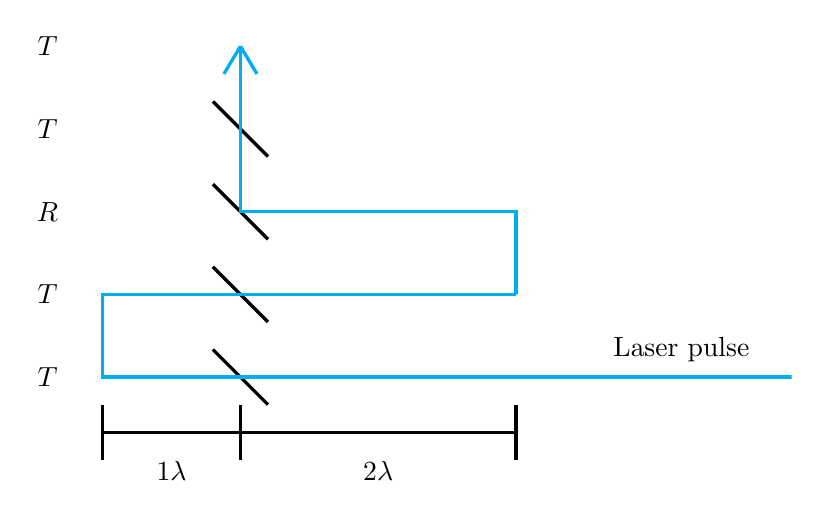
\begin{tikzpicture}[scale=0.7]
		%\node[] at (\labels, 5.5) {Behavior through splitter};
		\node[] at (\labels,6.0) {$T$};
		\node[] at (\labels,4.5) {$T$};
		\node[] at (\labels,3.0) {$R$};
		\node[] at (\labels,1.5) {$T$};
		\node[] at (\labels,0.0) {$T$};
		
		\draw[very thick] (10.5,\sone) -- (9.5,\sone+1); % Splitter 1
		\draw[very thick] (10.5,\stwo) -- (9.5,\stwo+1); % Splitter 2
		\draw[very thick] (10.5,\sthree) -- (9.5,\sthree+1); % Splitter 3
		\draw[very thick] (10.5,\sfour) -- (9.5,\sfour+1); % Splitter 4
		
		\draw[cyan, very thick] (\delayoneleft,0.0) -- (20.0,0.0) % Incoming pulse line
		to(\delayoneleft,0.0) -- (\delayoneleft,\delayvertical) % Delay Leg 1 (a)
		to(\delayoneleft,\delayvertical) -- (15,\delayvertical); % Pulse after delay 1
		
		\draw[cyan,very thick] (\mycenter,\delayvertical*2) -- (\delaytworight,\delayvertical*2)
		to(\delaytworight,\delayvertical) -- (\delaytworight,\delayvertical+1.5)
		to(\mycenter,\delayvertical*2) -- (\mycenter,\delayvertical*4);
		
		\draw[cyan, very thick] (9.7,5.5) -- (10.0,6.0); % arrow head left
		\draw[cyan, very thick] (10.0,6.0) -- (10.3,5.5); % arrow head right
		
		\node[] at (18,0.5) {Laser pulse};
		
		\node[] at (8.75,-1.7) {$1\lambda$};
		\draw[black, very thick] (\delayoneleft, -1) -- (\delaytworight, -1);
		\draw[black, very thick] (\delayoneleft, -1.5) -- (\delayoneleft, -0.5);
		\draw[black, very thick] (\mycenter, -1.5) -- (\mycenter, -0.5);
		
		\node[] at (12.5,-1.7) {$2\lambda$};
		\draw[black, very thick] (\delaytworight, 3.0+\buffer) -- (\delaytworight, 4.0+\buffer);
		
		\end{tikzpicture}
	\end{center} 
	\caption{Example of a laser pulse path through multisplitter. T indicates when the laser pulse is 
		transmitted through the splitter, and R stands for when the laser pulse is reflected by the splitter. 
		The operating wavelength is $\lambda = \SI{23}{cm}$. Bends are accomplished with two UV mirrors, 
		one at each corner of the delay line.}
	\label{fig:tikz}
\end{figure*}


Each splitter reduces the intensity of the pulse as a new pulse is generated. Expected intensities
can be predicted by using the measured T/R values for each splitter. For example, using $T/R=55/45$,
in Fig~\ref{fig:tikz} the laser pulse is transmitted four times and reflected once: 
\begin{equation}\label{eq:i4}
I_4 =  T \cdot R \cdot T \cdot T \cdot T \cdot I_0 \approx 0.41 I_0
\end{equation}
Therefore, this pulse would have a fairly high laser intensity, because it was transmitted multiple times. 
In the worst case, the laser pulse could be reflected ($45\%$) three times and transmitted ($55\%$) twice. 
\begin{equation}\label{eq:i6}
I_6 =  T \cdot R \cdot R \cdot R \cdot T \cdot  I_0 \approx 0.28 I_0
\end{equation}
This pulse would have a lower intensity when compared to the pulse traveling the path described in Equation~\ref{eq:i4}.
These trends were reflected in the electron bunch trains generated in the gun.
As a result, it was necessary to investigate methods to improve the intensity distribution. 

\Subsection{New UV Splitters}
To improve the intensity distribution, splitters with a tolerance of $50\%\pm3\%$ were purchased, 
installed, and the laser energy was measured again. The quality of the splitters was near tolerance 
again, and the bias leaned toward reflection, $T/R \approx 47/53$. With the bias now reversed, 
the trend in intensity distribution was also reversed. The possibility of using a combination 
of splitters from the $\pm3\%$ and $\pm5\%$ sets was explored. 
Using a python script to compare all possible combinations, it was determined that using only 
$\pm3\%$ splitters would result in the lowest variation in intensity. 

\Subsection{Train Intensity Measurements}
The train intensity for an eight pulse laser train was measured using the $\pm5\%$ and $\pm3\%$ splitters.
A train of sixteen will be used for TBA experiments, but eight was chosen for these measurements to
simplify the experimental set up, and reduced interruption to beam time 
runs which were using the four splitter set up. 
\begin{figure}%[h]
	\begin{center}
		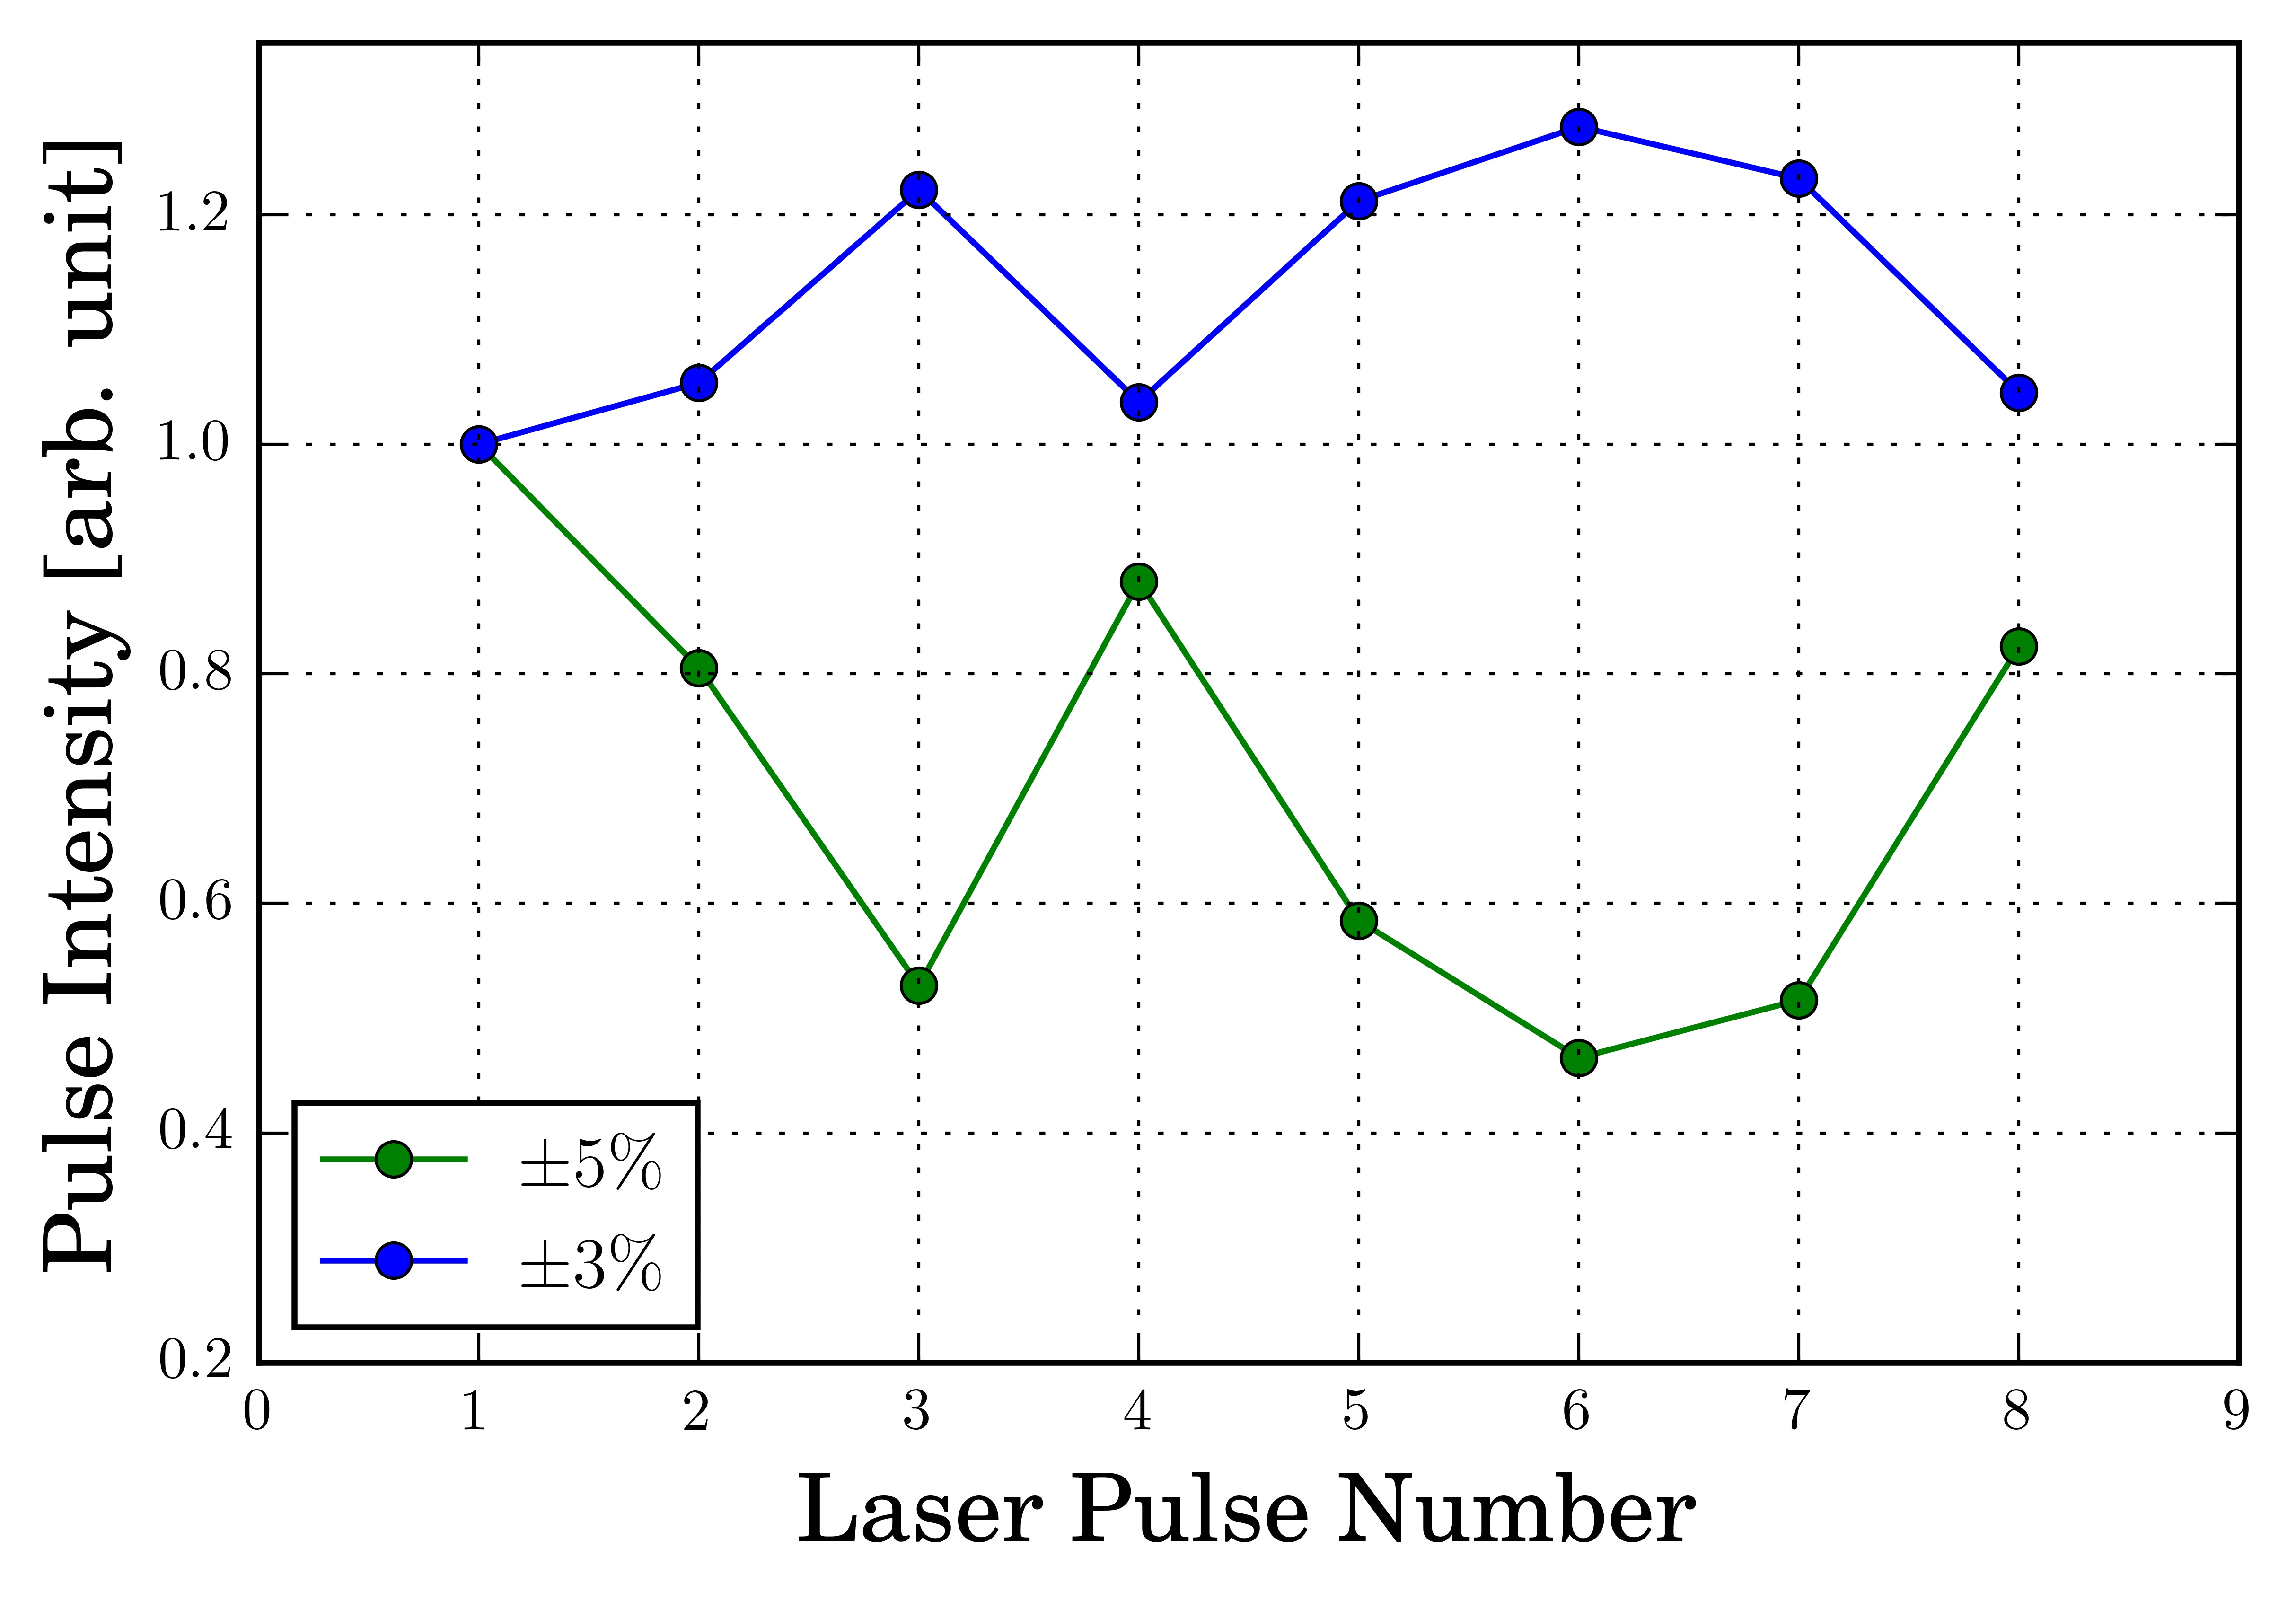
\includegraphics[width=0.75\textwidth]{images/splitter_improvement}
		\caption{Measurements of the laser pulse train intensity. The laser pulse number refers to 
			each pulse of light generated by the laser. These will respectively become electron bunch 1, 2, 3, and so on
			in the bunch train.}\label{fig:origtrain}
	\end{center}
\end{figure}
Equations~\ref{eq:i4} and~\ref{eq:i6} don't account for mirror losses in the delay legs, 
a lower value is expected in experimental measurments. The path of laser pulse one and
pulse four in the train can be described by an updated version of Equation~\ref{eq:i4}.
The number of splitters is reduced to four, and both pulses are transmitted three 
times and reflected once: 
\begin{align}
I_1 = R \cdot T \cdot T \cdot T \cdot I_0 \\
I_4 = T \cdot T \cdot R \cdot T \cdot I_0 
\end{align}

With about $\pm10\%$ mirror loss in the delay legs, we expect laser pulse one and four 
to be roughly the same intensity. This prediction matches the experimental measurements 
shown in Figure~\ref{fig:origtrain}. With the same 
logic, we expect pulse six to have the largest deviation from pulse one, as it is reflected 
three times and transmitted once in the four splitter set up. This expectation is also 
confirmed by the results in Figure~\ref{fig:origtrain}.  

While still not perfect, the laser pulse train is now more uniform.
Through the use of optics with tighter specifications and sorting of the optical elements, 
an improvement in laser pulse uniformity of 16.5\% was achieved.
This results in more uniform electron bunch trains, which means bunches 
of similar charge are delivered down stream. 
Since the power output in the PETS is a function of charge and bunch length, 
increased uniformity in the bunch train furthers the goals of TBA 
by helping provide more consistent power output from the PETS.

%%%%%%%%%%%%%%%%%%%%%%%%%%%%%%%%%%%%%%%%%%%%%%%%%%%%%%%%%%%%%%%%%%%%%%%%%%%%%%%%%%%%%%%%%%%%
%%%%%%%%%%%%%%%%%%%%%%%%%%%%%%%%%%%%%%%%%%%%%%%%%%%%%%%%%%%%%%%%%%%%%%%%%%%%%%%%%%%%%%%%%%%%
\Section{RF Measurements}
%%%%%%%%%%%%%%%%%%%%%%%%%%%%%%%%%%%%%%%%%%%%%%%%%%%%%%%%%%%%%%%%%%%%%%%%%%%%%%%%%%%%%%%%%%%%
%%%%%%%%%%%%%%%%%%%%%%%%%%%%%%%%%%%%%%%%%%%%%%%%%%%%%%%%%%%%%%%%%%%%%%%%%%%%%%%%%%%%%%%%%%%%

In order to accurately simulate the RF fields in the cavities on the drive and witness line, 
a set of detailed measurements were done to determine the power in each RF cavity.
These measurements are important, for several reasons. 
First, there are limited records at the AWA of these values in the past.
It is also important to know the ratio of power in each cavity w.r.t. the other cavities.
Ideally each cavity would be supplied the same amount of power, 
but as with all experimental hardware, the waveguide network is not ideal.
Two or more cavities are fed by one klystron which requires a network of 
power splitters and attenuators. If the power is split exactly, the ratio 
of power delivered to each cavity may be different. 
The amount of attenuation in the subsequent waveguide after the spitter could
also be the source of power difference at the cavities.
 
In an effort to understand these differences, 
power measurements of the drive gun, and linac tanks 
one through six on the drive line were taken.
The sections below detail the calibration used during power measurements and the 
resulting values that informed simulations. 

\Subsection{Cable Calibration} \label{cablecal}
There is a significant length of cable that connects the cavities to the control room.
Since no cable is a perfect conductor, they do add attenuation to any signal propagated
and measured after the cables.
This attenuation needs to be accounted for so that the power measurements 
taken are not misleading. The cable effects can be taken into account
by comparing a reference single supplied directly to the power meter
versus the reference single passed through the cables and then supplied to the power meter.
To do this comparison, a signal generator was placed in the tunnel, see Figure~\ref{fig:signalgenerator}. 
Then a signal was propagated to the control room where it was 
measured and compared to the original power measurement in the tunnel, see Figure~\ref{fig:tikzcalibration}. 
\begin{figure*}%[h]
	\begin{center}	
		\begin{circuitikz}[scale=0.7]
            \draw (0,0) to[csV=] (2,0);
            \node[align=center] at (0.8,2.0) {Signal \\ Generator};
            
			%Control room or power meter
			\def \leftside {3}
			\def \topbox {0.75}
			\def \botbox {-0.75}
			\draw (2.0, 0) -- (\leftside, 0);
			\draw[fill=white, ultra thick, rounded corners =0.1cm] (\leftside,\botbox)rectangle  
			({\leftside+3},\topbox) node[pos=0.5, align=center] {Meter};           
		\end{circuitikz}
    \end{center} 
\caption{Refrence power reading was taken while power meter was directly connected to the 
signal generator. The resulting power was $P_s=\SI{-8.92}{dBm}$}
\label{fig:signalgenerator}
\end{figure*}
\def \delayvertical {1.5}
\iftrue
\begin{figure*}%[h]
	\begin{center}	
		\begin{circuitikz}[scale=0.7]
			
			\draw (0,0) to[csV=] (2,0);
			\node[align=center] at (0.8,2.0) {Signal \\ Generator};
			%Short blue RF cable 
			\node[] at (3.5,1) {$C_{1}$};
			\node[tlinestub] at (2,0){};
			\node[] at (3.5,-1) {};
			
			%Long RF cable
			\node[] at (7,1) {$C_{2}$};
			\node[tlinestub] at (5.5,0){};
			
			%Short yellow RF cable
			\node[] at (9.5,1) {$C_{3}$};
			\node[tlinestub] at (8.1,0){};
			%\draw[] (4.6,0) to[short,-] ++(1,0);
			\draw (4.6, 0) -- (5.6, 0);
			%10 dB attenuator
			\draw (10.7,0) to[R=$\SI{10}{dB}$, color=red] (14,0);
			
			%Control room or power meter
			\def \leftside {14}
			\def \topbox {0.75}
			\def \botbox {-0.75}
			%\draw (10.75, 0) -- (\leftside, 0);
			\draw[fill=white, ultra thick, rounded corners =0.1cm] (\leftside,\botbox)rectangle  
			({\leftside+3},\topbox) node[pos=0.5, align=center] {Meter};
		\end{circuitikz}
	\end{center} 
	\caption{Experimental set up when calibrating the cables from gun to control room. 
		Where $C_1$ is a short blue heliax, $C_2$ is a long heliax to the control room, 
		and $C_3$ is a short yellow heliax to the 6 GHz scope or power meter.}
	\label{fig:tikzcalibration}
\end{figure*}
\fi

The power reading in the control room was $P_c = \SI{-9.48}{dBm}$, and the power reading in 
the tunnel from the signal generator was $P_s = \SI{-8.92}{dBm}$, so the
attenuation is $\SI{0.56}{dB}$. However, one more cable needs to be accounted for and 
subtracted from the overall attenuation. A short blue heliax was used to connect the 
signal generator to the control room cables, as shown in Figure~\ref{fig:tikzcalibration}.
This cable not normally connected to the control room as shown in Figure~\ref{fig:tikzdrivegun}. 
\lsnote{You should finish the thought - how much attenuation from the Heliax, and what is the adjusted correction?}


\Subsection{Drive Gun Measurements}\label{gunenergy}
After the cable calibration, the set up was returned to typical rf conditions as 
shown in Figure~\ref{fig:tikzdrivegun}. This includes $\SI{53.2}{dB}$ from the pick 
up probe itself, a $\SI{36}{dB}$ additional attenuation connected to the 
drive gun pick up probe, followed by a long heliax to the 
control room. The signal split in the control room with a mini-circuit ZFRSC-123-S+. 
Links to the specification sheets of all splitters used in this chapter can be found in Appendix~\ref{rf}.
One port is used for Low Level RF (LLRF) control, and the other port was connected to a short 
heliax, $C_3$, then to a $\SI{10}{dB}$ attenuator and finally to the 
power meter. Normally a load is placed at port two when no power meter is connected. 
Next, the klystrons and phase shifters were set to supply 
maximum power to the gun, typical of TBA running conditions. 
\def \delayvertical {1.5}
\iftrue
\begin{figure*}%[h]
	\begin{center}		
		\begin{circuitikz}[scale=0.7]
			\def \leftside {17.0}
			\def \topbox {0.75}
			\def \botbox {-0.75}
			
			\node[] at (0.8,1.3) {Gun};
			\draw (0,0) to[csV=] (2,0);
			
			\def \gunright {2}
			%Attenuators
			%\node at (2, -0.50) {$P_1$};
			%\node at (5, -0.50) {$P_2$};
			
			\draw (\gunright,0) to[R=$\SI{53.2}{dB}$, color=red] (\gunright+2,0);
			\draw (\gunright+2.5,0) to[R=$\SI{36}{dB}$, color=red] (\gunright+4.5,0);
			\draw[] (\gunright+2.0,0) to[short,-] ++(0.5,0);
			%Long RF cable
			
			\node[] at (\gunright+6,1) {$C_{2}$};
			\node[tlinestub] at (\gunright+4.5,0){};
			\draw (9.0, 0) -- (10.0, 0);
			\draw[fill=white, ultra thick, rounded corners =0.1cm] (\gunright+8.0,\botbox)rectangle  
			%splitter
			({\gunright+11.0},\topbox) node[pos=0.5, align=center] {Splitter};
			\draw (11.5, 0.7) -- (11.5, 2);
			\node[] at (11.5, 2.5) {LLRF};
			
			%Short yellow RF cable
			\draw (13.0, 0) -- (13.5, 0);
			\node[] at (\gunright+13.0,1) {$C_{3}$};
			\node[tlinestub] at (\gunright+11.5,0){};
						
			%10 dB attenuator
			\draw (16.0, 0) -- (16.5, 0);
			\draw (\gunright+14.5,0) to[R=$\SI{10}{dB}$, color=red] (\gunright+16.5,0);
			
			%Control room or power meter
			\draw (18.5, 0) -- (\leftside+2, 0);
			\draw[fill=white, ultra thick, rounded corners =0.1cm] (\leftside+2,\botbox)rectangle  
			({\leftside+5},\topbox) node[pos=0.5, align=center] {Meter};
		\end{circuitikz}
	\end{center} 
	\caption{Experimental set up when measuring power from gun to control room. 
		Where $\SI{53.2}{dB}$ of attenuation is due to the gun probe itself, 
		$\SI{36}{dB}$ of additional attenuation is attached to gun pick up probe cable in the tunnel, 
		$C_2$ is a long heliax to the control room. The $\SI{9.5}{dB}$  splitter sends half the signal to the   
		low level RF (LLRF) control system, and half to the power meter. 
		$C_3$ is a short yellow heliax that connects the meter to the splitter and on to the 6 GHz scope or power meter.}
	\label{fig:tikzdrivegun}
\end{figure*}
\fi

Using the set up in Figure~\ref{fig:tikzdrivegun}, the power meter measured  $P_{g} = \SI{-14.18}{dBm}$
in the control room. Now we must account for attenuation to know the true power
signal out of the gun. \lsnote{ {\it Did you ever compare to Eric's measurement?}}
\nrnote{\it He did not take direct power measurements. He measured the power supplied by the 
klystrons, which would not be effected by differences in the power splitters or 
attenuation in the waveguide as it travels to the cavity. }
\begin{equation}
P_g =P_{meas}- \left(P_r + A_1 + C_2 + S + C_3 + A_2 \right)
\end{equation}
Where A's represent attenuators, C's represent cable calibration numbers.
\begin{equation*}
\begin{aligned}
P_g \, \SI{}{[dBm]} = \\
\SI{53.2}{dB} + \SI{36}{dB} + \SI{0.56}{dB} \\
 + \SI{9.5}{dB}+ \SI{0.56}{dB} + \SI{10}{dB} + \SI{14.18}{dBm} \\
 = \SI{124}{dBm} or 95.6?
\end{aligned}
\end{equation*}

Then converting to a more convenient unit: 
\begin{equation}
P \, \SI{}{[dBm]} = 10 \cdot \log{\frac{P \, \SI{}{[mW]}}{\SI{1}{[mW]}}}
\end{equation}
\begin{equation} \label{eq:dbmtomw}
P \, \SI{}{[mW]} = \SI{1}{[mW]} \cdot 10^{\frac{P \, [\SI{}{dBm}]}{\SI{10}{}}}
\end{equation}
\begin{equation} 
P_2 = 10^{\SI{9.56}{dBm}} \cdot  \SI{1}{[mW]} = 3.6 \, \SI{}{[MW]} 
\end{equation}

\Subsection{Linac Cavity Measurements}
\lsnote{{\it Need intro sentences.  Why do this?}}
There are six linear accelerating (linac) cavities after the gun. 
Each are connected to the control room in the same way as the gun. 
The only differences are in the attenuation at the pick up probe and 
the splitter attenuation. Using the methods in section \ref{gunenergy}, 
and the attenuation values, we can calculate the power in each linac cavity:
\lsnote{There are missing values in table}
\begin{table} %or [hbt] ?
	\caption{\label{tab:powerlinac} Power and attenuation values for the 
		linac cavities. Note that all cavities have an additional 
		\SI{33}{dB} attenuation added after the probe.}
	\begin{center}
		\begin{tabular}{ccccc}
			\toprule
			\toprule
			\textbf{Cavity} & \textbf{Probe Att.} & \textbf{Splitter Att.} & \textbf{Power Meter 1}  & \textbf{Power Meter 2} \\
			\midrule
			Gun & \SI{-53.2}{dB}& $9.5 \pm \SI{0.3}{dBm}$ & \SI{-14.18}{dBm} & \SI{-3.86}{dBm}  \\
			2 & \SI{}{dB}       & $9.5 \pm \SI{0.3}{dBm}$ & \SI{-18.88}{dBm} & \SI{-9.6}{dBm}  \\
			3 & \SI{}{dB}       & $4.0 \pm \SI{1.0}{dBm}$ & \SI{-12.24}{dBm} & \SI{-1.54}{dBm}  \\
			4 & \SI{-61.95}{dB} & $9.5 \pm \SI{0.3}{dBm}$ & \SI{-18.89}{dBm} & \SI{-10.11}{dBm}  \\
			5 & \SI{}{dB}       & $9.5 \pm \SI{0.3}{dBm}$ & \SI{-17.76}{dBm} & \SI{-8.39}{dBm}  \\
			6 & \SI{-61}{dB}    & \SI{}{dB} 			  & \SI{-14.32}{dBm} & \SI{-2.83}{dBm} \\
			\bottomrule
		\end{tabular}
	\end{center}
\end{table}

\begin{equation}
P_1 = \SI{-61.95}{dBm} + \SI{33}{dB} + \SI{0.56}{dB} + \SI{9.5}{dBm} +\SI{10}{dBm}
\end{equation}

\lsnote{Concluding sentences.  What is significance of your measurement?}

\Section{Beam diagnostics}

\lsnote{You need an intro for the diagnostics section.  What beam measurements need to be done for TBA and optimization studies, and what are the corresponding diagnostics?  Describe what will follow.}

%%%%%%%%%%%%%%%%%%%%%%%%%%%%%%%%%%%%%%%%%%%%%%%%%%%%%%%%%%%%%%%%%%%%%%%%%%%%%%%%%%%%%%%%%%%%
%%%%%%%%%%%%%%%%%%%%%%%%%%%%%%%%%%%%%%%%%%%%%%%%%%%%%%%%%%%%%%%%%%%%%%%%%%%%%%%%%%%%%%%%%%%%
\Section{Energy Measurements} \label{sec:dipolecal}
%%%%%%%%%%%%%%%%%%%%%%%%%%%%%%%%%%%%%%%%%%%%%%%%%%%%%%%%%%%%%%%%%%%%%%%%%%%%%%%%%%%%%%%%%%%%
%%%%%%%%%%%%%%%%%%%%%%%%%%%%%%%%%%%%%%%%%%%%%%%%%%%%%%%%%%%%%%%%%%%%%%%%%%%%%%%%%%%%%%%%%%%

Energy measurements at the AWA are done with a dipole 
spectrometer magnet. The set up includes two Yittrium 
Aluminum Garnet (YAG) screens as shown in Fig~\ref{fig:spectrometer}.

\begin{figure*}%[h]
	\begin{center}		
		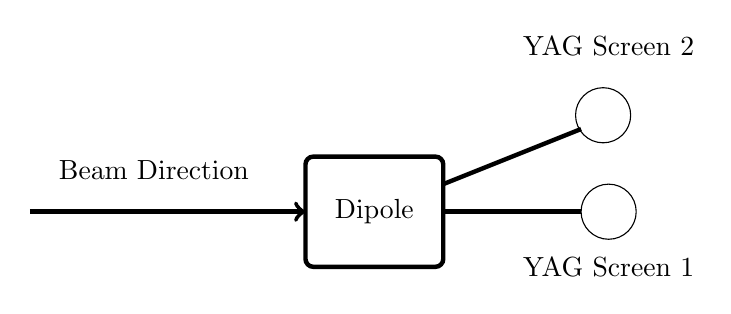
\begin{tikzpicture}[scale=0.7]
			
			\node[] at (2.25,0.75) {Beam Direction};
			\draw[ultra thick, ->] (0,0) -- (5.0, 0.0);
			
			\draw[fill=white, ultra thick, rounded corners =0.1cm] (5.0,1.0)rectangle  
			(7.5,-1.0) node[pos=0.5, align=center] {Dipole};
			
			\draw[ultra thick] (7.5, 0.0) -- (10.0, 0.0);
			\draw[ultra thick] (7.5, 0.5) -- (10.0, 1.5);
						
			\node[] at (10.5, 3) {YAG Screen 2};
			\draw (10.4,1.75) circle (0.5cm);
			
			\node[] at (10.5, -1.0) {YAG Screen 1};
			\draw (10.5,0) circle (0.5cm);
			
		\end{tikzpicture}
	\end{center} 
	\caption{Spectrometer set up in all cases at AWA.}
	\label{fig:spectrometer}
\end{figure*}

\Subsection{Energy Measurement Procedure}
Taking an energy measurement requires a beam trajectory
that is centered through the preceding quadrupole magnets. Otherwise, the beam 
may experience unintentional steering from the quadrupole magnets, and possibly excessive non-uniform fields 
if it enters the dipole off-axis. The centering is checked by powering the two 
quads before the dipole. The center is found by focusing 
in the x-direction, and then the y-direction. If the beam 
moves horizontally or vertically as it is being focused, 
the quad is "steering", because the beam is entering the magnets off-axis.
Once the beam is centered through the quads on YAG screen 1, 
the dipole is then turned on to bend the beam.
The two YAG screens are positioned so that when the dipole is off, 
a centered beam will hit YAG screen 1. When the dipole is turned
on, the beam is made to appear at the center of YAG screen 2 corresponding to a 
beam bent $20^\circ$. In this way, the dipole strength needed to center the beam and YAG screen 2 can 
then be used to determine the beam energy.

\Subsection{Energy Calculation}
Based on the procedure above, there is one number which is used to back calculate the mean energy. The current
supplied to the dipole is determined by the number of "counts"
keyed into the control system. A counts to current conversion
is calculated based on the measurements shown in Table \ref{tab:counts}.  \lsnote{{\it This table reference is not right}}
\begin{table}
\begin{center}
	\caption{Counts to current data for the first dipole in the drive beam line.}
	\label{tab:counts}
\end{center}
	\begin{tabular}{c c} 
		\toprule
		\toprule
		Counts & Current [A] \\ [0.5ex] 
		\midrule
		1000 & 3.7 \\ 
		
		5000 & 18.8 \\
		
		10000 & 37.5 \\
		
		15000 & 56.3 \\
		\bottomrule
		
	\end{tabular}
\end{table}
Then the B-field is calculated given the current: 
\begin{equation}
	\SI{}{B\,[T]} = (180.9708\cdot \SI{}{I\,[A]} - 7.2053)\cdot 10^{-4}
\end{equation}
There are a few geometric calculations that need to be done using the magnetic field value. 
before we can calculate the energy. 
The radius of curvature, $\rho$, 
can be calculated using the effective length of the dipole, L, and bending angle, $\theta$.
\begin{equation}
	\rho = \frac{L}{2\cdot \sin(\frac{\theta}{2})}
\end{equation}
\lsnote{{\it Starting here, the derivation below is hard to follow.  I am still not sure how you got eq. 2.11.  Then, eq. 2.12 needs more explanation, at least units in the proper places.  Eq. 2.13 seems to be missing a `c' in the momentum term.}}
Using $\rho$, and geometry, we can also estimate the x offset of the
beam after the dipole: 
\begin{equation}
	\Delta x = \rho \left( 1- \cos\theta \right)
\end{equation}
Using this and the famous relationship, $B\rho$ \cite{Wiedemann},
we can relate the B field and the beam momentum. 
\begin{equation}
	\SI{}{p\,\left[\frac{MeV}{c}\right]} = \frac{B\cdot \rho}{3.3356}\cdot 10^3
\end{equation}
We can then calculate the total energy by including the rest mass of the electrons \cite{Griffiths}:
\begin{equation}
	\SI{}{E\,[MeV]} = \sqrt{0.511^2+p^2}
\end{equation}\label{eq:energy}

\Subsubsection{Hard Edge Dipole Example}
\begin{figure*}
	\begin{center}		
		\begin{tikzpicture}[scale=1]
		\node (fig1) at (0,0)
		{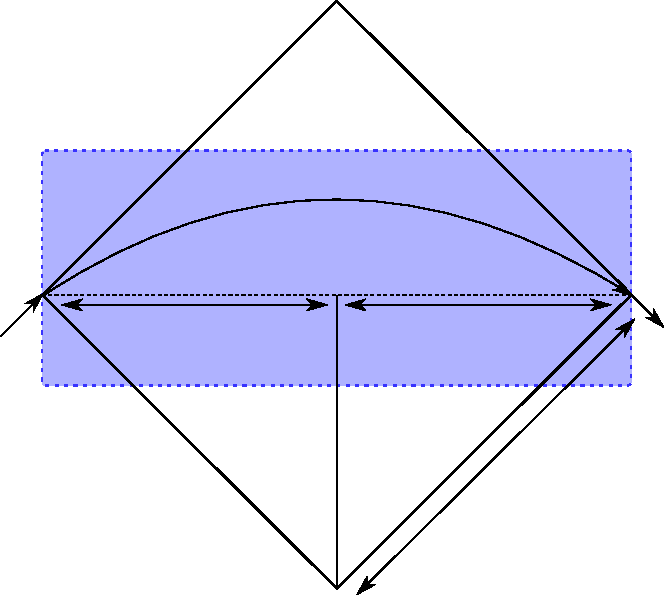
\includegraphics[width=0.5\textwidth]{./images/dipole_geometry}};
		\node[fill=white, inner sep=2pt] (txt2) at (-1.25,0.5) {$\frac{L}{2}$};
		\node[fill=white, inner sep=2pt] (txt2) at (-0.5,-2) {$\frac{\theta_k}{2}$};
		\node[fill=white, inner sep=2pt] (txt2) at (0.7,-2) {$\frac{\theta_k}{2}$};
		\node[fill=white, inner sep=2pt] (txt2) at (1.25,0.5) {$\frac{L}{2}$};
		\node[fill=white, inner sep=2pt] (txt2) at (2.5,-2) {$\rho$};
		\end{tikzpicture}
	\end{center} 
	\caption{Simplified drawing of the beam trajectory through a dipole with a uniform field. }
\end{figure*}\label{fig:dipole-geometry}
\lsnote{{\it I do think a numerical example is appropriate here}}
\nrnote{this example is more of a double check and reference for me than for the reader...}
Since this calculation is used several time throughout the 
beam line for different magnets, lets consider a hard edge 
dipole, to show how the above equations can be used to determine
the x offset after the magnet, and the beam energy. 

Let's define the dipole length, $L=\SI{0.2}{[m]}$, angle, $\theta=\SI{20}{degrees}$. 
The corresponding radius is $\rho = \SI{0.5759}{[m]}$. With these values we can now 
calculate the offset, $\Delta x \approx \SI{34}{[mm]}$, which is confirmed by OPAL. 

\nrnote{not sure if I want to include energy since it depends on measured counts....}
Given a count of  energy of $\SI{64.8}{[MeV]}$ given measured counts of 

%%%%%%%%%%%%%%%%%%%%%%%%%%%%%%%%%%%%%%%%%%%%%%%%%%%%%%%%%%%%%%%%%%%%%%%%%%%%%%%%
%%%%%%%%%%%%%%%%%%%%%%%%%%%%%%%%%%%%%%%%%%%%%%%%%%%%%%%%%%%%%%%%%%%%%%%%%%%%%%%%
\Section{Transverse Beam Size Measurements} \label{sec:beamsize}
%%%%%%%%%%%%%%%%%%%%%%%%%%%%%%%%%%%%%%%%%%%%%%%%%%%%%%%%%%%%%%%%%%%%%%%%%%%%%%%%
%%%%%%%%%%%%%%%%%%%%%%%%%%%%%%%%%%%%%%%%%%%%%%%%%%%%%%%%%%%%%%%%%%%%%%%%%%%%%%%%

\lsnote{Intro - why beam size measurements needed?}
Beam size measurements are taken by using YAG screens at multiple z locations along the beam line.
The code used to produce all the following images can be found at this git repository: 
\url{https://github.com/nneveu/imageProcessing}

\Subsection{Capturing Images}
\nrnote{Add tikz picture here to show how camera is pointed into beam line with mirrors}\\
Raw YAG screen images can vary widely depending on the camera set up, charge, and 
light in the room. In some cases the edges of the YAG screen are illuminated as shown in Figure~.
The focal distance is also different for every camera and depends on the camera and mirror
locations inside and outside of the vacuum chambers.
\lsnote{include some actual YAG images}

\Subsection{Post Processing Images}
A python script was written to take beam images and convert them to profiles in the x and y direction.
This is done in a series of steps, and requires that one or more images can be used as a 
background image and fiducial image. A background image must capture any dark current 
that is present when the beam is not hitting the YAG screen. The fiducial image must 
clearly show the edges of the YAG screen so that a mm/pixel conversion can be calculated.
The following steps detail the post processing from raw image to transverse beam size estimate.

\Subsubsection{Step 1: Calculating the fiducial}

\Subsubsection{Step 2: Remove background intensity}

\Subsubsection{Step 3: Calculate x and y beam profile}

\Subsubsection{Step 4: Fit profile to calculate beam size}


\Section{Bunch Length Measurements}\label{sec:bunchlength}

Must have line break here.\\
\lsnote{Intro: why needed?}

\Subsection{Measurement Technique}
In order to measure the bunch length, we performed an autocorrelation scan
of the Coherent Transition Radiation (CTR) produced by the electron distribution \cite{Happek, WBarry}.
\lsnote{{\it Also, describe how CTR produced}} In brief, the CTR is transported into a Michelson interferometer (MI)
where it's split and directed into two MI arms with a half-transparent pellicle \cite{PhysRevSTAB.9.082801}. 
The CTR beams are then combined together at the exit of the MI with the variable path difference.
The resulting CTR intensity is registered with a liquid helium cooled IR Labs
bolometer \cite{bolo} as a function of path difference.
The path difference is then converted into time as $\Delta \tau = 2 \Delta x$.
The resulting FWHM bunch duration is determined from the Gaussian fit of 
the interferogram; see Figure~\ref{interferogram}.
\begin{figure}
	\centering
	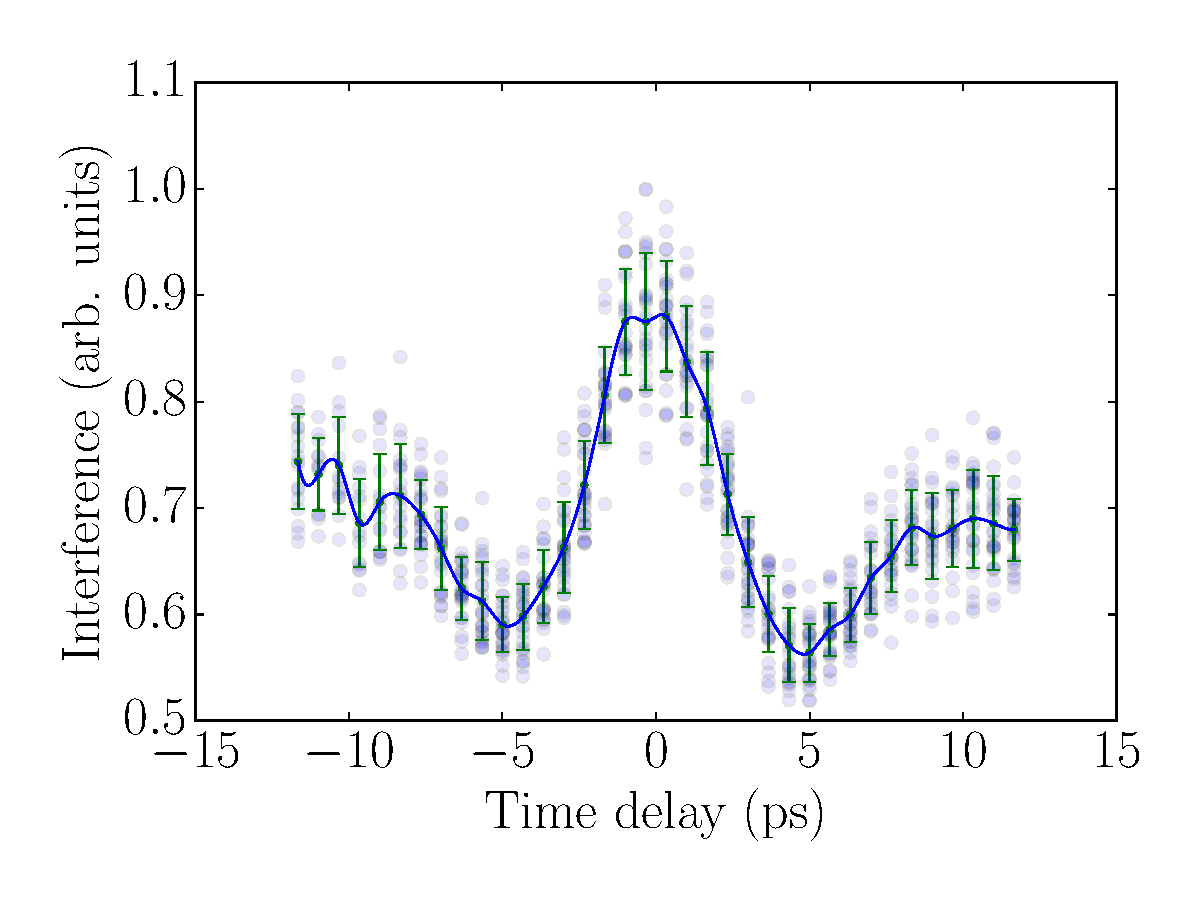
\includegraphics[width=0.75\linewidth]{images/THPMF048f1}
	\caption{An example interferogram for Q=30 nC and laser pulse FWHM of 1.5 ps.}
	\label{interferogram}
\end{figure}
To alleviate the effect of charge fluctuations, we recorded 15 bolometer values for each data point.
The values were then averaged and the error bars were deduced from the data. The data points
outside of the 3$\sigma$ bracket were considered as outliers and discarded. The resulting
interference pattern as a function of time delay in the MI is similar to that presented in Figure~\ref{interferogram}.

\begin{figure*}%[hbt]
	\centering
	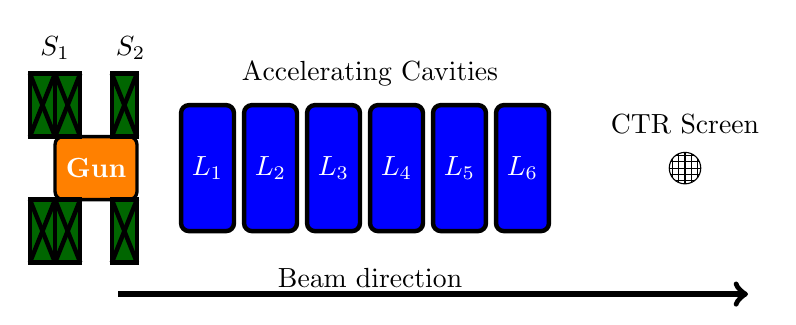
\begin{tikzpicture}[scale=0.8, text=black]
	\def \gunleft {-1.0}
\def \gunright {0.3}
\def \loneright {1.0}
\def \ltworight {2.0}
\def \lthreeright {3.0}
\def \lfourright {4.0}
\def \lfiveright {5.0}
\def \lsixright {6.0}
\def \quadone {7.5}

%Line between kicker and septum
\node[] at (4.0,-0.75) {Beam direction};
\draw[line width=0.75mm, ->] (0.0,-1.0) -- (10,-1.0);

\draw[fill=orange, very thick, rounded corners =0.1cm] (\gunleft,0.5)rectangle (\gunright,1.5) node[pos=.5, white] {\textbf{Gun}} ;
%S1
\node[] at (-1,2.9) {$S_1$};
\draw[ultra thick, fill=black!60!green] (-1.4,-0.5)rectangle  (-1.0,0.5) node[pos=.5, white] {} ;
\draw[black, ultra thick] (-1.4,-0.5) -- (-1.0,0.5);
\draw[black, ultra thick] (-1.4,0.5) -- (-1.0,-0.5);
\draw[ultra thick, fill=black!60!green] (-1.4,1.5)rectangle  (-1.0,2.5) node[pos=.5, white] {} ;
\draw[black, ultra thick] (-1.4,1.5) -- (-1.0,2.5);
\draw[black, ultra thick] (-1.4,2.5) -- (-1.0,1.5);
%S2
\draw[ultra thick, fill=black!60!green] (-1.0,-0.5)rectangle  (-0.6,0.5) node[pos=.5, white] {} ;
\draw[black, ultra thick] (-1.0,-0.5) -- (-0.6,0.5);
\draw[black, ultra thick] (-1.0,0.5) -- (-0.6,-0.5);
\draw[ultra thick, fill=black!60!green] (-1.0,1.5)rectangle  (-0.6,2.5) node[pos=.5, white] {} ;
\draw[black, ultra thick] (-1.0,1.5) -- (-0.6,2.5);
\draw[black, ultra thick] (-1.0,2.5) -- (-0.6,1.5);

%S3
\node[] at (0.2,2.9) {$S_2$};
\draw[ultra thick, fill=black!60!green] (-0.1,-0.5) rectangle  (0.3,0.5) node[pos=.5, white] {};
\draw[black, ultra thick] (-0.1,-0.5) -- (0.3,0.5);
\draw[black, ultra thick] (-0.1,0.5) -- (0.3,-0.5);
\draw[ultra thick, fill=black!60!green] (-0.1,1.5) rectangle  (0.3,2.5) node[pos=.5, white] {};
\draw[black, ultra thick] (-0.1,1.5) -- (0.3,2.5);
\draw[black, ultra thick] (-0.1,2.5) -- (0.3,1.5);
%Linac drawings 
\node[] at (4,2.5) {Accelerating Cavities};
\draw[fill=blue, ultra thick, rounded corners =0.1cm] (\loneright,0)rectangle  ({\loneright+0.84},2) node[pos=.5, white] {$L_1$} ;
\draw[fill=blue, ultra thick, rounded corners =0.1cm] (\ltworight,0)rectangle  ({\ltworight+0.84},2) node[pos=.5, white] {$L_2$};
\draw[fill=blue, ultra thick, rounded corners =0.1cm] (\lthreeright,0)rectangle ({\lthreeright+0.84},2) node[pos=.5, white] {$L_3$};
\draw[fill=blue, ultra thick, rounded corners =0.1cm] (\lfourright,0)rectangle ({\lfourright+0.84},2) node[pos=.5, white] {$L_4$};
\draw[fill=blue, ultra thick, rounded corners =0.1cm] (\lfiveright,0)rectangle ({\lfiveright+0.84},2) node[pos=.5, white] {$L_5$};
\draw[fill=blue, ultra thick, rounded corners =0.1cm] (\lsixright,0)rectangle ({\lsixright+0.84},2) node[pos=.5, white] {$L_6$};

%current optimization point
%\node[draw, fill=yellow, star, star points=5, star point ratio=0.6, minimum size=0.1cm]
%at (12.5,1.0) {$z_1$};
\node[] at (9,1.7) {CTR Screen};
\clip[draw] (9,1) circle (0.25cm);
\draw[step=1mm] (-1,-1) grid (10,10);

%Line between kicker and septum
\draw[very thick] (13.25,0.2) -- (14.5,-0.5);


%Line between septum and dipole
\draw[very thick] (15.6,-0.5) -- (16.5,-0.5);




	\end{tikzpicture}	
	\caption{Beam line layout at the AWA.}
	\label{beamline}
\end{figure*}
\Subsection{Experimental Setup}
The beam line layout is shown in Figure~\ref{beamline}. 
Bunches were allowed to propagate freely to the 
CTR screen. The only focusing elements used were solenoids $S_1$ and
$S_2$. As the bunches passed the CTR screen, light was
emitted through a window located next to the screen, 
as shown in Figure~\ref{bolo}. A slit was used to prevent
background x-rays from reaching the bolometer.
After passing the slit, the CTR propagated to the 
interferometer also shown in Figure~\ref{bolo}.  \lsnote{{\it This section would benefit from a block diagram of the set up}} 
A remotely movable stage inside the interferometer was swept, 
and the resulting combined signal fed to the bolometer. 
%The bolometer was cooled with liquid helium. 
Periodic refilling of the helium is required when taking data in order
to keep the bolometer at \SI{4}{K}. The bolometer sensitivity knob for studies included in this work was at position ``1'' and
the gain set to 200.
For the case of 1 nC electrons beams, the laser transverse profile was homogenized prior to the vacuum injection \cite{PhysRevAccelBeams.20.103404}.
To produce high-charge 30 nC beams, we implemented an additional laser beamline that bypasses the homogenizer due to the losses in the 
MLA and relay optics.

\begin{figure}
	\centering
	\begin{tikzpicture}[every node/.style={anchor=south west,inner sep=0pt},x=1mm, y=1mm,]   
	\node (fig1) at (0,0)
	{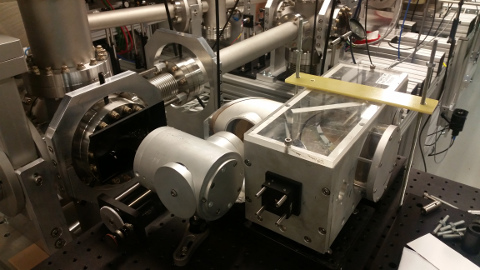
\includegraphics[width=0.5\textwidth]{images/THPMF048f3}};
	\node[fill=white, inner sep=2pt] (txt2) at (35,15) {Interferometer};
	\node[fill=white, inner sep=2pt, rotate=26] (txt2) at (18,19.5) {Slit};	
	\node[fill=white, inner sep=2pt, rotate=20] (txt2) at (13,27) {Window};
	
	\node (fig2) at (0,-50)
	{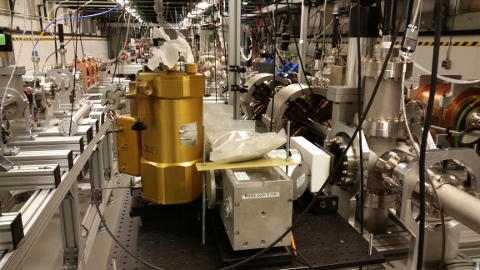
\includegraphics[width=0.5\textwidth]{images/THPMF048f4}};
	\node[fill=white, inner sep=2pt] (txt2) at (35,-42) {Interferometer};	
	\node[fill=white, inner sep=2pt] (txt2) at (55,-25) {Window};	
	\node[fill=white, inner sep=2pt] (txt2) at (22,-15) {Bolometer};
	\end{tikzpicture}
	\caption{IR labs bolometer and MI interferometer used in the experiment
		to capture CTR light as it exited a window on the beam line. }
	%\label{inter}
	%\caption{Bolometer. }
	\label{bolo}
\end{figure}

\lsnote{ Here, instead of sim discussion, have modification for independent staging, and previous energy gain measurement.}


\Section{AWA Design Requirements} \label{sec:requirements}

\lsnote{{\it Not sure if this section should be here, or later, more toward end of chapter.  This section is probably where you should have the overview of simple staging versus full staging, and a summary of what was required to go to full staging.  The title of the section should also be changed, maybe `Fully staged two beam acceleration'?  Probably need another (or repeated) figure here.}}


% An example for enumerate
\begin{enumerate}
	\item Kicker Design
	\item Septum Design
	\item Optimization 
\end{enumerate}

% A quotation example
% Every quota must be accompanied by a reference to the source
% in a footnote or in the Bibliography
\begin{quotation}
	test
\end{quotation}




\Section{Chapter Summary}

Line break.

